\documentclass[10pt,a4paper,onepage,DIV12]{scrartcl}
% \areaset{210mm}{297mm}
\usepackage[T1]{fontenc}        %k.A.
\usepackage[latin1]{inputenc} %k.A.
%\usepackage{ngerman}   %Deutsch
\usepackage{amssymb,amsmath,amsthm}     %Mathe
\usepackage[pdftex]{graphicx} %Bilder
% \usepackage[german]{babel}
\usepackage[usenames,dvipsnames,pdftex]{color}
\usepackage[english]{babel}
\usepackage[font=small,labelfont=bf]{caption}
%\usepackage{bibgerm}
%\usepackage{subfig}
%\usepackage[subfigure]{tocloft}
\usepackage{xstring}
\usepackage[colorlinks=true]{hyperref}
\setlength{\headheight}{15pt}
\usepackage{fancyhdr}
\usepackage{listings}
\usepackage{svn-multi}
\svnidlong
{$HeadURL$}
{$LastChangedDate$}
{$LastChangedRevision$}
{$LastChangedBy$}
\usepackage{url}
\newcommand{\svnloc}{\StrBefore[5]{\svnkw{HeadURL}}{/}}


\usepackage{multicol}
\lstset{language=Matlab
, basicstyle=\ttfamily\scriptsize\bfseries
, keywordstyle=\color{Blue}\pmb
, breaklines=true
, commentstyle=\color{OliveGreen} 
, 
}
\lstset{numbers=left, stepnumber=2, numberstyle=\tiny, numbersep=5pt
%, frame=tb
}

\pagestyle{fancy}
\fancyhf{}
\lhead[\thepage]{Correlation procedure for CLEM -- Rev. \svnrev}
\rhead[\leftmark]{\thepage}

\title{Correlative Microscopy - Algorithm overview}
\author{Martin Schorb, \href{mailto:martin.schorb@embl.de}{martin.schorb@embl.de}}


\publishers{\small{\vspace{2mm} corresponds to revision \svnrev\; commited at \svndate}\\\small{ of \texttt{martin\_correlate.m} at 
\svnloc}}

\setlength{\columnsep}{10pt}

\begin{document}
 \maketitle
\section{Introduction}
This document describes the usage of the algorithms designed for correlation of fluorescence microscopy images to their corresponing EM image.\\

The correlation procedure, as described in Kukulski et al.,2011 JCB, consists of two major coordinate transformations. The first one uses fluorescent microspheres to calculate the mapping of a single point fluorescent signal onto an electron microscopy image of low resolution ($4-10 $k$\times$). The obtained coordinates can then be transformed further using a different fiducial system (in this case the gold beads used for tomogram reconstruction) to a high magnification image.\\

This document provides a step by step manual in how to use the algorithms, their parameters and outputs and shows the corresponding code snippets to give an idea of the points at which certain things happen while running the script.
\section{Installation and requirements}

\subsection{System and software requirements}A MATLAB\textsuperscript{\textregistered} 
installation version 7.4.0 onwards including the Image Processing Toolbox is required for succesfully running the scripts. This should be independent on the type of operating system used. However the function was so far only successfully tested on Linux and Mac OS X 10.4  environments. 
\\

In order to access the newest version of the scripts, a subversion (SVN\footnote{See \url{http://www.structures-it.embl.de/services/online/vcs},\; \url{http://en.wikipedia.org/wiki/Subversion}}) client is needed. It is usually included in most Linux distributions and easy to obtain for other operating systems. In case you don't have access to a software capable of checking out subversion repositories, you can simply download all files individually from the webserver (\url{https://svn.structures/repo/schorb:Corr}).


\subsection{Obtaining the newest version of the correlation algorithms}
The main scripts as well as all supporting underlying algorithms and this documentation are stored in a central subversion repository which is accessible from within the EMBL network.
\subsubsection*{First installation}
To checkout the most recent version of algorithms and documentation files for the first time, create a directory where you want to store these files. 

Then checkout the files to this directory using your subversion client. The Unix Terminal command will be this:
\begin{verbatim}
 svn checkout https://svn.structures/repo/schorb:Corr /your/directory/
\end{verbatim}
Accept the encryption certificate (permanently) by pressing \texttt{p}.\\

You should see a result similar to this:
\begin{verbatim}

A    Corr/martin_contrast.m 
A    Corr/martin_correlate.m
...
A    Corr/martin_tfm_beads.m
Checked out revision 56.

\end{verbatim}

Now you have a local working copy of the most recent versions of the correlation files.\\

Add this directory including all subdirectories to the MATLAB path by adding the following line to MATLAB's \texttt{startup.m} script, that is usually located in a MATLAB related folder within your home directory (\texttt{$\sim$/.matlab/startup.m}) when working in a Linux environment. 
\begin{verbatim}
 addpath (genpath('/path/to/your/directory'),'-begin')
\end{verbatim}
On Macintosh or Windows systems you have to add the path by using MATLAB's preferences. Make sure that also the subdirectories are added.\\
\subsubsection*{Updating your existing scripts}

To have your scripts and documentation files always up to date according to the current revision, update them from the repository by simply executing
\begin{verbatim}
 svn up
\end{verbatim}
 in the directory in which you put the scripts.\\ 


If you receive an error message this most likely means that you've edited some of the scripts yourself and thus there's a conflict resulting, because the file you want to update from the server is different than what the program expects. Most of the time giving \verb|tf| as response to the conflict will solve the issue. If not, save your initialization script to another directory and delete the entire script directory (including all hidden files). Then perform a clean new installation of the scripts as described above.

\subsubsection*{Editing the scripts}
You are able manipulate and edit your local working copy of the scripts (activate or remove sub-pixel fitting, shift correction etc.). However these changes will be reverted while updating to a newer revision. \textcolor{red}{Therefore please be really cautious while doing this! Use the initialization script instead to personalize the correlation procedure or let me know if there's substantial changes that you need.}\\

Also note that there will be some hidden files and directories (\texttt{.svn} etc.) written while checking out. These contain important information needed by subversion and should not be modified or deleted.

\subsubsection*{Initialization}

You can adjust key parameters of the correlation scripts by modifying the initialization script as shown below. When checking out the repository a file called \texttt{corr\_init\_orig.m} will appear. You can simply rename this filie to \texttt{corr\_init.m} and change the parameters and paths according to your needs. This file will then stay in your local scripts directory and will not be overritten while updating the scripts with the newest version from the repository.\\

\begin{quote}\textcolor{red}{
   It might occur that in future revisions additional parameters will be added to this script, so in case you run into an error message stating this, just update your local \texttt{corr\_init.m} with the changes you find in the downloaded and most up-to-date \texttt{corr\_init\_orig.m}.}
 \end{quote}
 \lstinputlisting[]{../corr_init_orig.m}
\newpage
\section{Correlation from LightMicroscopy to LowMag EM image}

Correlation from the original fluorescence image to an appropriate EM image containing indentifiable fiducial markers is performed using the script \texttt{martin\_correlate}.

\subsection{Executing the script}
To execute the script and start the correlation simply run \begin{verbatim}
 martin_correlate(fmf,emf,gmf,rmf,outfileroot)
\end{verbatim}
 in the MATLAB command line.
 \lstinputlisting[linerange={1-8}]{../martin_correlate.m}
It requires the following input parameters:
\begin{enumerate}
 \item\texttt{fmf} -- path to FM image file containing fiducial information (1344$\times$1024 pixel, 8 or 16bit tiff-file)
 \item\texttt{emf} -- path to EM image file containing visible fiducials (2048$\times$2048 pixel, 8 or 16bit tiff-file)
 \item\texttt{gmf} -- path to FM image file containing point of interest in first channel -- considered to be GFP (same dimensions and format as fmf)
 \item\texttt{rmf} -- path to FM image file containing point of interest in second channel -- considered to be RFP (same dimensions and format as fmf)
 \item\texttt{outfileroot} -- directory and name base for generating output files.
\end{enumerate}
\newpage
\subsection{Output and generated files}
\label{sec:lm_output}
The following files are generated by the correlation script during runtime. The name base is referred to as \texttt{BASE}. An appended \texttt{XFP} refers to the fluorescent channel chosen for correlation. The selected correlation that was used is denoted by either the transform number or \texttt{all} in case the transformation based on all beads was chosen (\texttt{\#}). 
\begin{itemize}
 \item \texttt{BASE\_picked1.txt} -- Plain text file containing the coordinates of fiducial pairs after subpixel fitting. \lstinputlisting[linerange={235-240}]{../martin_correlate.m}

\item \texttt{BASE.pickspots1.mat} -- Fiducial pair coordinates, input parameters, selected fluorescent channel and clicked fluorescence spot -- MATLAB format.\lstinputlisting[linerange={242-243}]{../martin_correlate.m}

 \item \texttt{BASE\_XFP\_fluoshift.shiftcoos.mat} -- Coordinates from bleed-through fiducials to determine shift in between the acquisition of images.(within \texttt{martin\_chromaticshift\_drift2} sub-script)
\lstinputlisting[linerange={41-41}]{../martin_chromaticshift_drift2.m}


\item \texttt{BASE\_XFP\_\#\_pred.tif} -- Overlay image showing the predicted and actual positions of the fiducials in EM coordinates. (size of EM-image, 16bit tiff-file)
\item \texttt{BASE\_XFP\_\#\_prediction.tif} -- Circle marking the position of the transformed coordinate of the spot of interest. (all images with same properties)
\item \texttt{BASE\_XFP\_\#\_pred\_overlay.tif} -- Overlay of the prediction circle and EM image
\item \texttt{BASE\_XFP\_\#\_fm.tif} -- Transformed fluorescent fiducial image 
\item \texttt{BASE\_XFP\_\#\_em.tif} -- electron microscopy image 
\item \texttt{BASE\_XFP\_\#\_gm.tif} -- Transformed image of first fluorescence channel (GFP)
\item \texttt{BASE\_XFP\_\#\_rm.tif} -- Transformed image of second fluorescence channel (RFP)
\item \texttt{BASE\_XFP\_\#\_tfmed.tif} -- Transformed fluorescence fiducial coordinates
\item \texttt{BASE\_XFP\_\#\_pickedem.tif} -- Picked EM coordinates

\item \texttt{BASE\_XFP\_\#.appltfm.mat} -- MATLAB data file storing transformed coordinates, selected fluorescence channel and paths to source files for further processing
\item \texttt{BASE\_XFP\_\#\_transform.log} -- Plain text log file containing the source files used for correlation, the transformed spot coordinates and various information about the used transformation
\end{itemize}

\newpage
\subsection{User interaction and key procedures}
\subsubsection{Contrast adjustment - optional}
If selected in the initialization script, the contrast of each fluorescent image can be adjusted. This is done using the script \verb|martin_contrast(image)| . The contrast can be adjusted either manually or automatically.
\begin{figure}
 \centering
 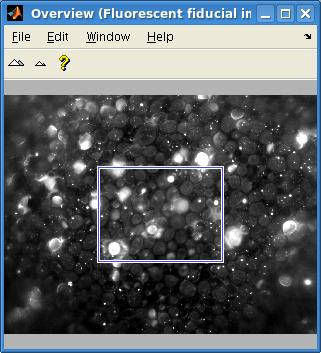
\includegraphics[width=0.2\textwidth]{images/contr_overview.jpg}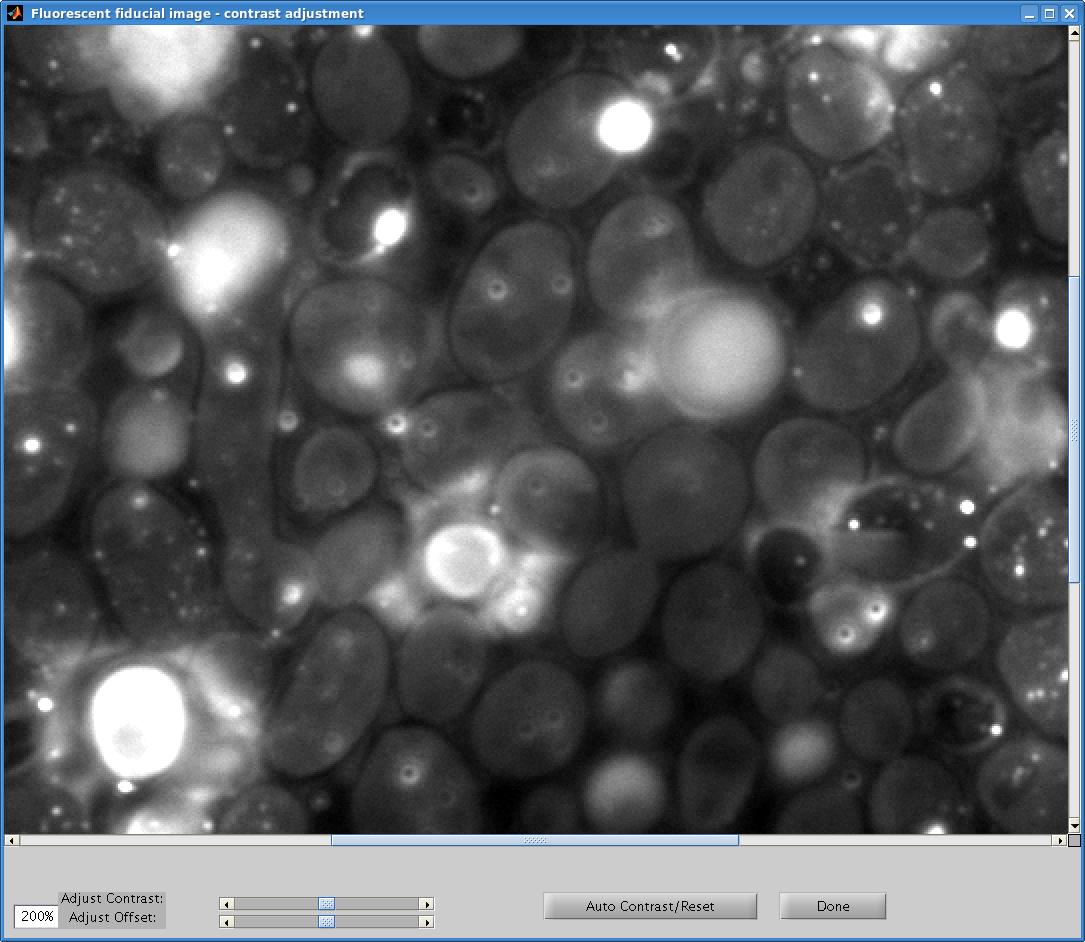
\includegraphics[width=0.65\textwidth]{images/contr.jpg}
 % contr.jpg: 1085x942 pixel, 762dpi, 3.62x3.14 cm, bb=0 0 103 89
 \caption{Contrast adjustment tool}
 \label{fig:contrast}
\end{figure}

A file selection dialog will ask to open already existing fiducial coordinate files. If the selected images have never been used for correlating before, just close that window.\\

\subsubsection{Rotation of the fluorescence fiducial image}
\label{sec:rotation}

If no previous fiducial coordinates could be found you can rotate the fluorecence fiducial image in 90 degree steps to simplify the initital detection of fiducial pairs.\,(Fig.\,\ref{fig:rotate}) Just rotate the image until its orientation fits best the EM-image presented in the small window.

\begin{figure}
 \centering
 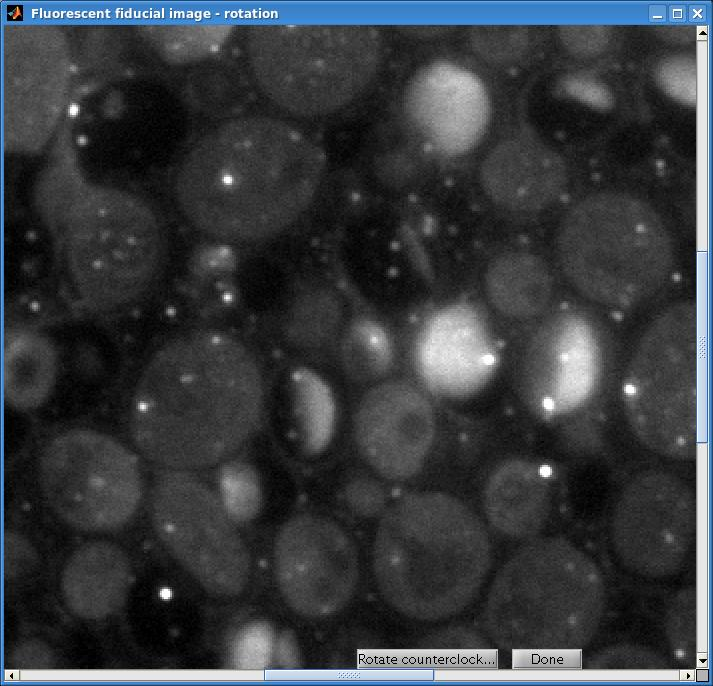
\includegraphics[width=0.65\textwidth]{images/rotate.jpg}
 % rotate.jpg: 713x686 pixel, 762dpi, 2.38x2.29 cm, bb=0 0 67 65
 \caption{Image rotation window for initial correlation}
 \label{fig:rotate}
\end{figure}

If the proper orientation is selected, click ``Done''. The initial manual assignment of fiducial pairs now is done with the selected orientation. For the further processing and coordinate checks the original orientation will be used.


\subsubsection{Fiducial selection}
\label{sec:fiducials}

Fiducial pairs are selected in both LM and EM image using the \texttt{cpselect} tool. When an already existing coordinate file is opened, these are displayed.\, (Fig.\,\ref{fig:cpsel_fid1}) To continue, close the window.

\begin{figure}
 \centering
 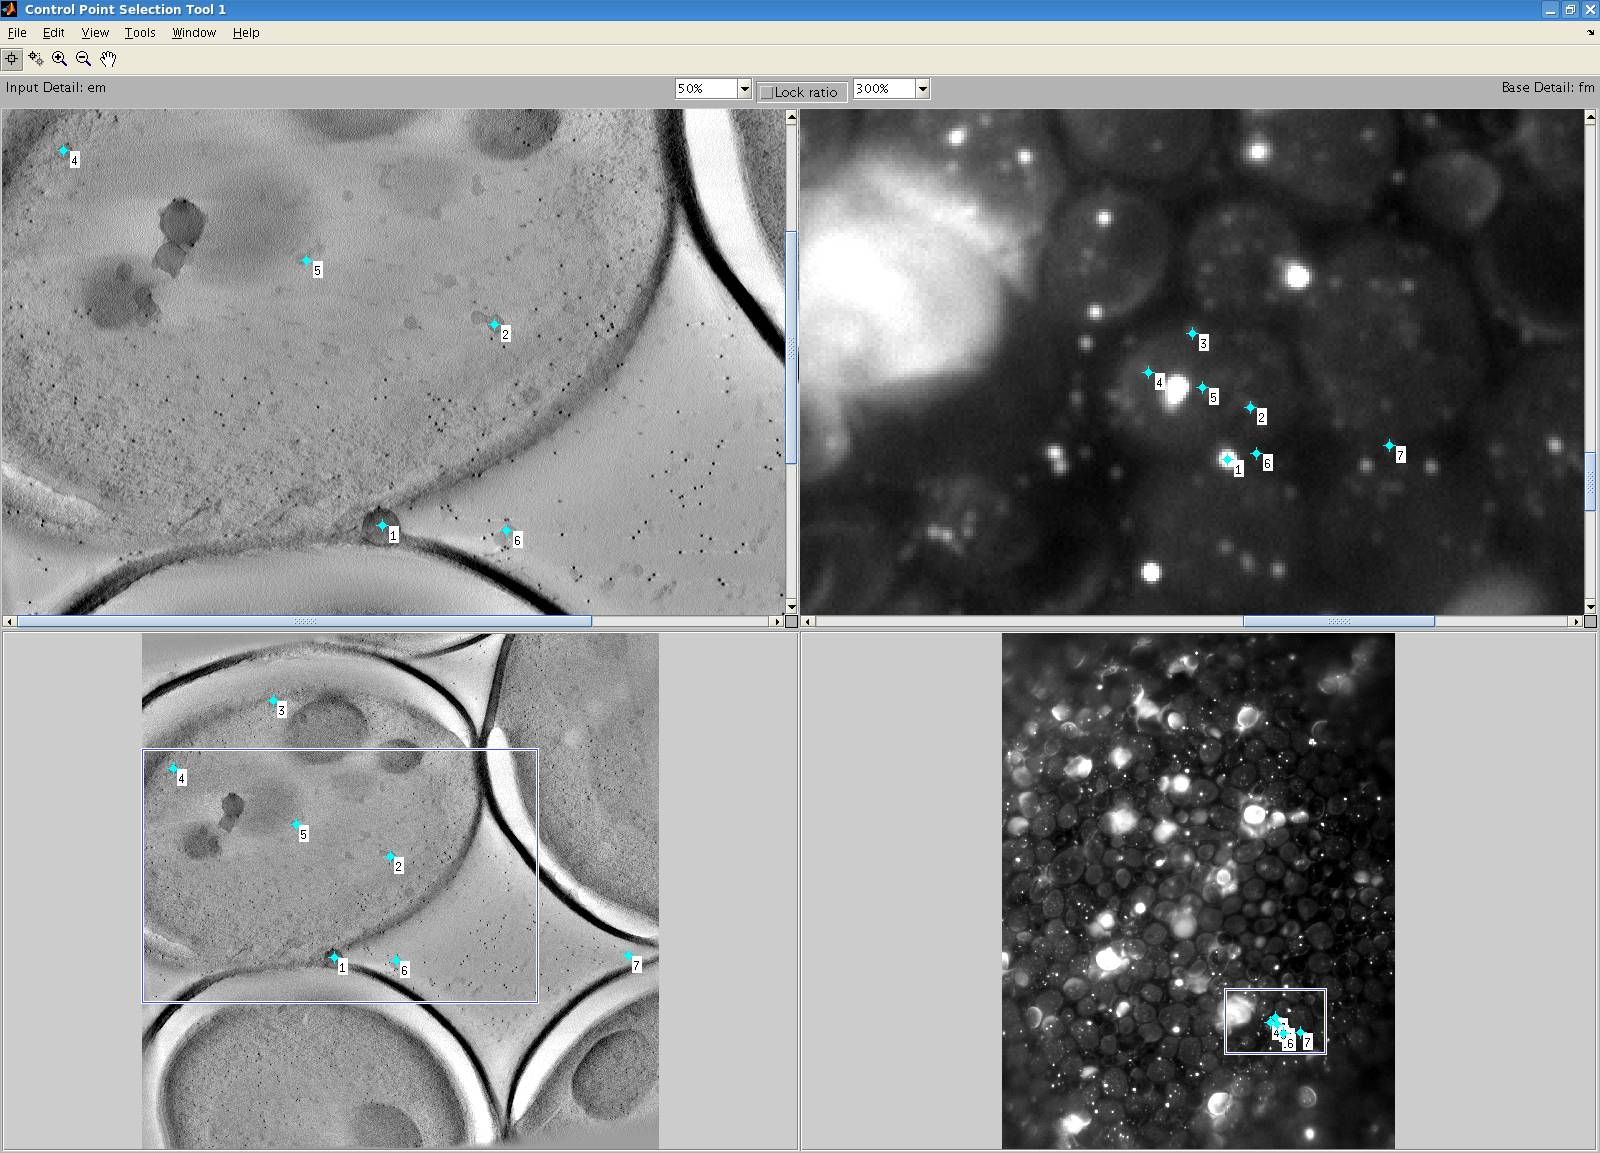
\includegraphics[width=.78\textwidth]{images/cpsel_fid1.jpg}
 % cpsel_fid1.png: 1600x1153 pixel, 72dpi, 56.44x40.68 cm, bb=0 0 1600 1153
 \caption{\texttt{cpselect} -- graphical interface for picking and checking fiducial positions}
 \label{fig:cpsel_fid1}
\end{figure}

\subsubsection{Fiducial sub-pixel fitting and display}
Fiducial positions in the light microscopy image are fitted with sub-pixel accuracy using a center of mass detection after high-pass filtering.
The fitted positions are presented again using a \texttt{cpselect} dialog.\,(Fig.\,\ref{fig:cpsel_fid1}) To continue, close the window.

 \lstinputlisting[linerange={157-157,205-206}]{../martin_correlate.m}

\subsubsection{Selection of fluorescence channel}
A popup window will ask you to determine the fluorescence channel in which your signal of interest is imaged.(Fig.\,\ref{fig:fluorsel})

\begin{figure}
 \centering
 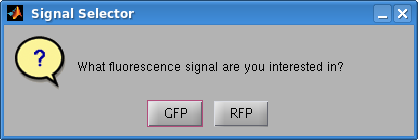
\includegraphics[width=.38\textwidth]{images/fluorsel.png}
 % fluorsel.png: 418x140 pixel, 72dpi, 14.75x4.94 cm, bb=0 0 418 140
\caption{graphical interface for selecting the fluorescence channel}
 \label{fig:fluorsel}
\end{figure}

\subsubsection{Picking the fluorescent spot of interest}
In the folowing \texttt{cpselect} dialog, the selected fluorescence image is shown on the right, the positions indicating the fiducial markers. Click once in the right image to determine the position of the spot of interest AND once in the left image just anywhere. This click in the left image will have no effect on the correlation. \texttt{cpselect} otherwise would just not export the clicked coordinates.\,(Fig.\,\ref{fig:cpsel_fluor1}) To continue, close the window. In case you forget to click in the left image, a reminder will be shown and you have the chance to click again. 
\begin{figure}
 \centering
 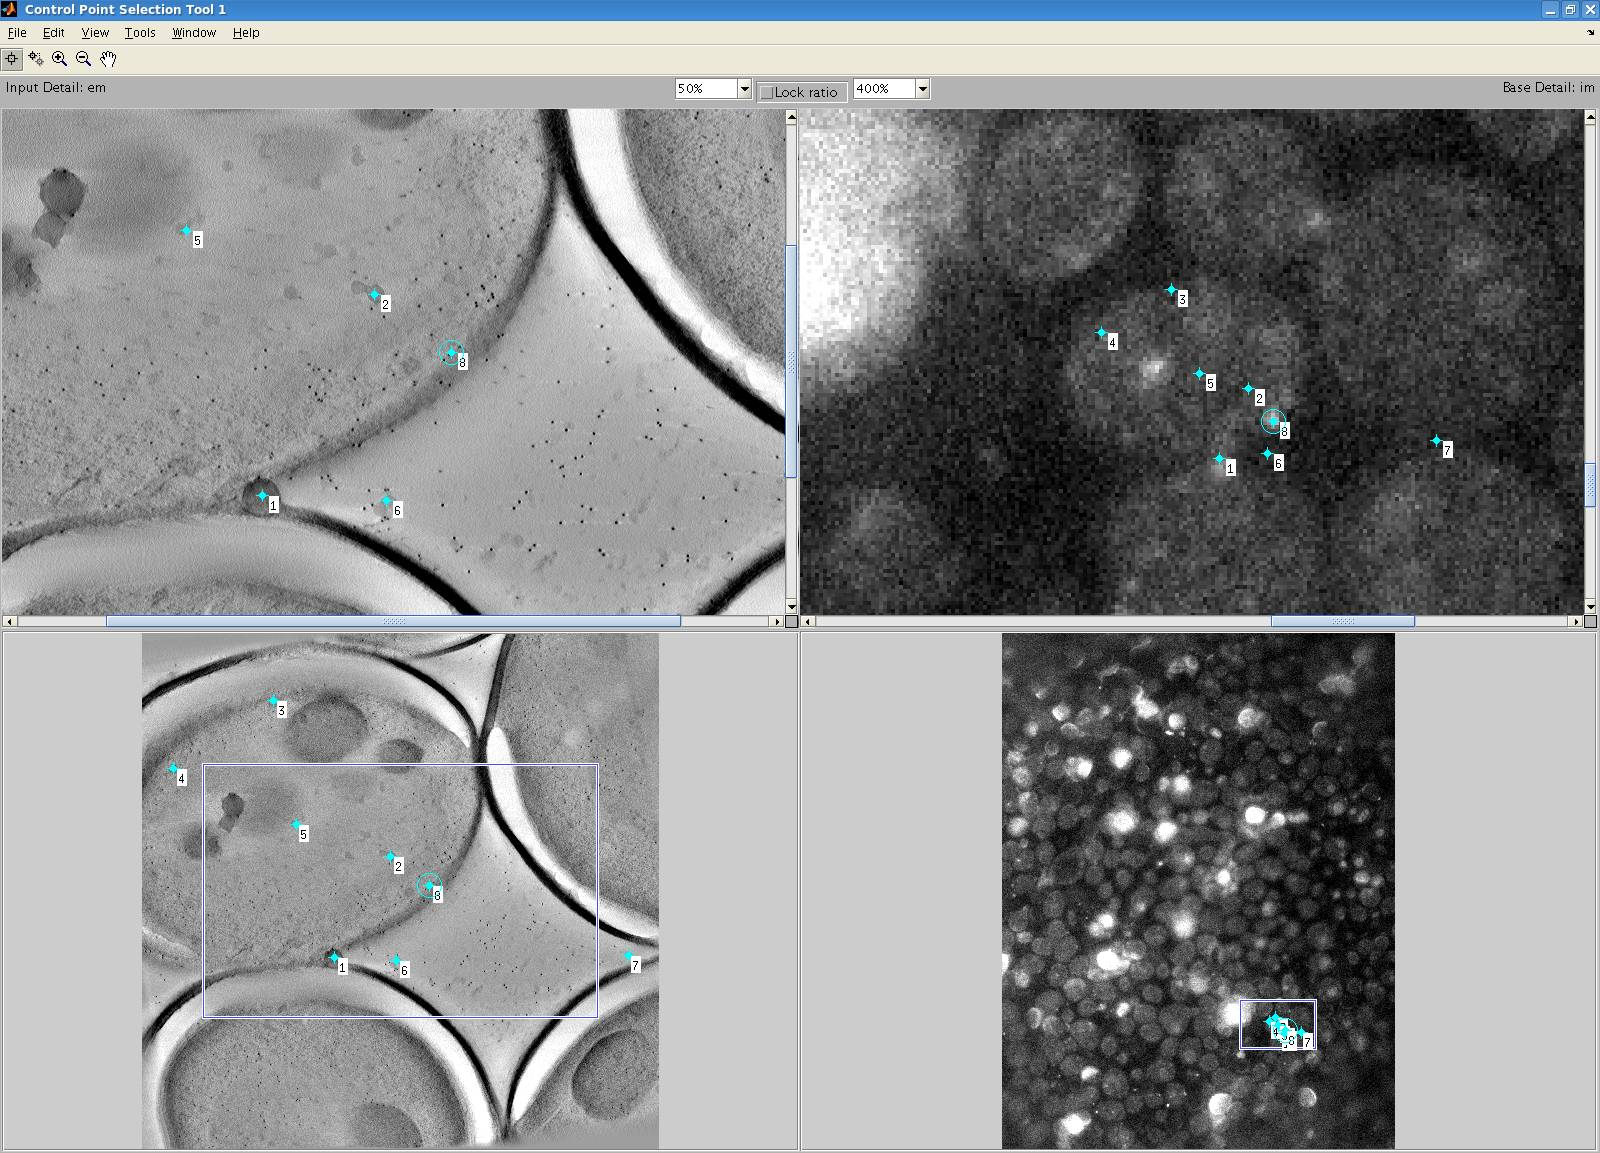
\includegraphics[width=.78\textwidth]{images/cpsel_fluor1.jpg}
 % cpsel_fluor1.png: 1600x1153 pixel, 72dpi, 56.44x40.68 cm, bb=0 0 1600 1153
 \caption{Selection of the fluorescent spot of interest -- marked spots \#8. The selected fluorescence channel image is shown on the right, the left click can be arbitrary.}
 \label{fig:cpsel_fluor1}
\end{figure}

\subsubsection{Sub-pixel fitting of the fluorescent spot of interest}
The coordinates of the fluorescent spot of interest are also determined by a centroid fit of the high-pass filtered image. The resulting coordinate will be presented in a new \texttt{cpselect} window. (Fig.\,\ref{fig:cpsel_fluor2})\\

To continue, close the window. 

\lstinputlisting[linerange={297-298,314-315}]{../martin_correlate.m}

\begin{figure}
 \centering
 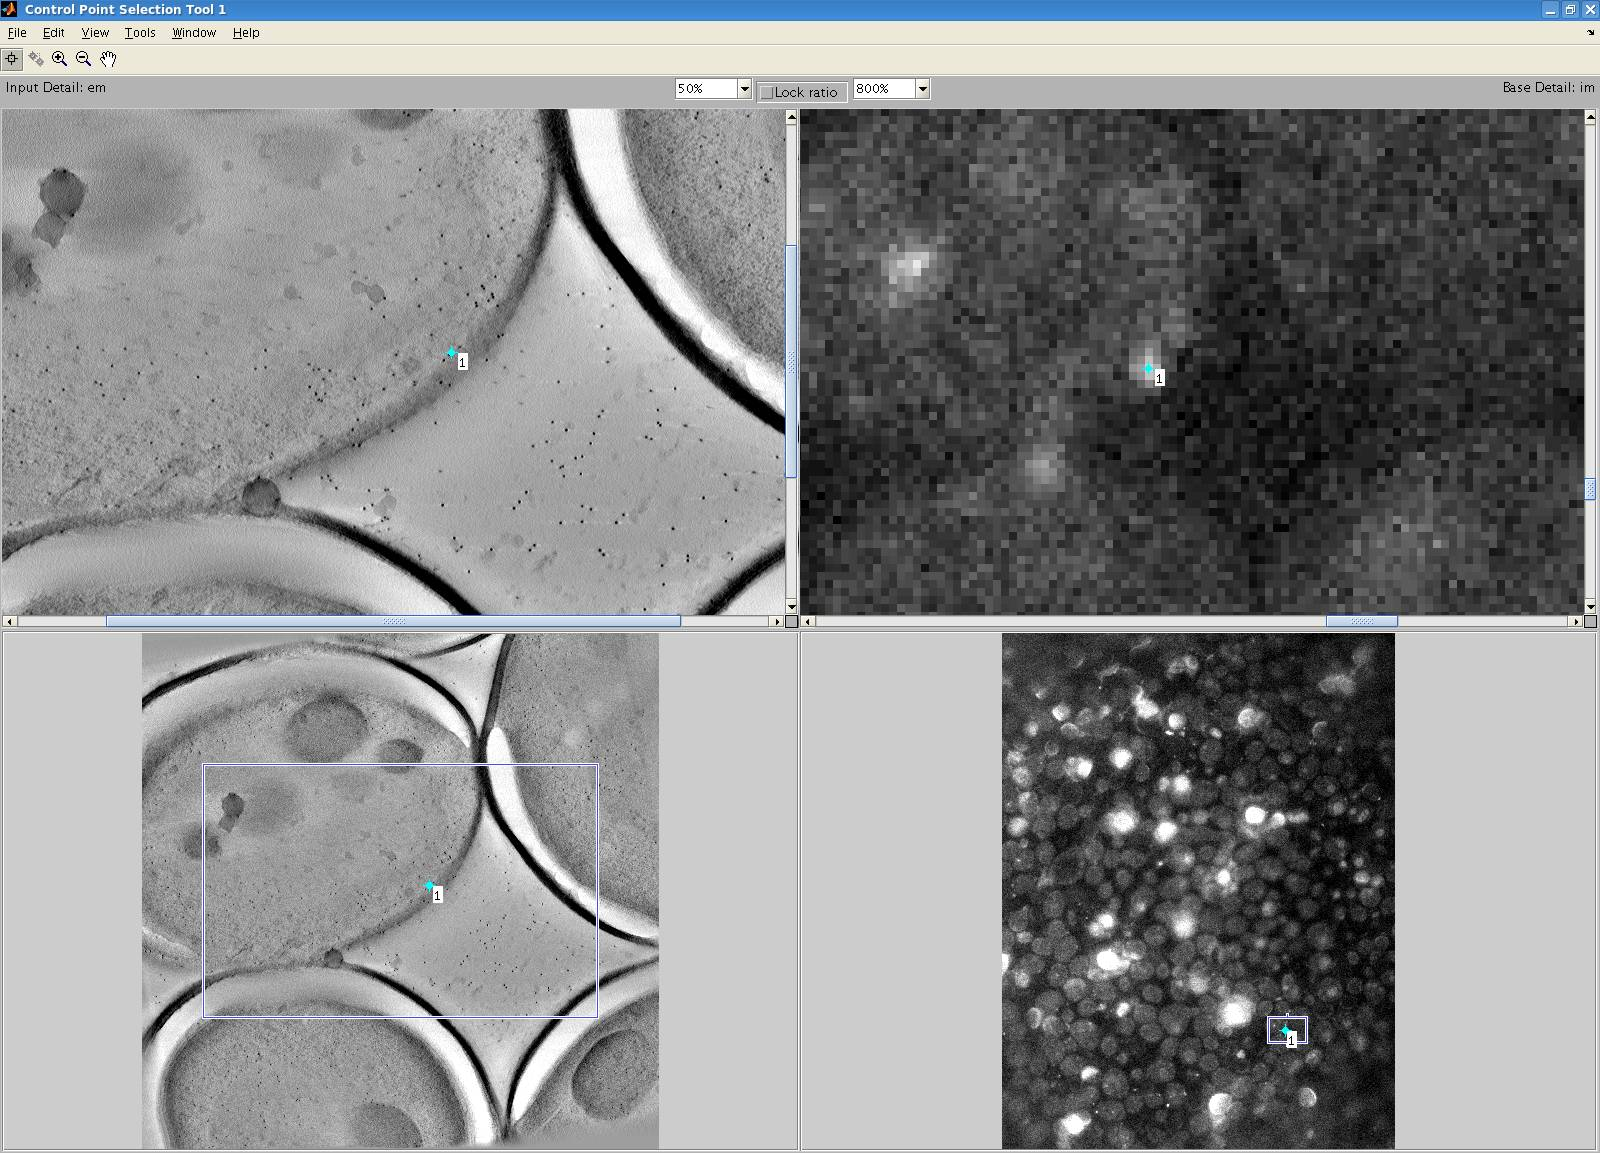
\includegraphics[width=.78\textwidth]{images/cpsel_fluor2.jpg}
 % cpsel_fluor2.png: 1600x1153 pixel, 72dpi, 56.44x40.68 cm, bb=0 0 1600 1153
 \caption{Positioning of the spot of interest after sub-pixel fitting.}
 \label{fig:cpsel_fluor2}
\end{figure}

\subsubsection{Correction of stage drift in between imaging of the different fluorescence channels}
The possible drift of the light microscope stage in between acquisition of the different flourescence images is accounted for using the fiducial signal that bleeds through into the longer wavelength channels. This step can be skipped if not needed. Just close the selection window and select ``Export and Close''. To continue then press any key while having the main MATLAB window active. If you constantly want to skip this correction you can modify your configuration script accordingly.\\

A file selection window will ask for already existing files storing these coordinates.\\

In case no pre-existing shift coordinates are selected a new window will open showing an RGB-overlay of the fiducial fluorescence image in red and the selected fluorescence channel containing the signal of interest in green. (Fig.\,\ref{fig:digitize}) % If a message window pops up stating that the variable called \texttt{XY} already exists, just choose overwriting it 
Click the obvious bleeding fiducials (both channels show a spot-like signal in close proximity) and close the window, saving the positions. If you cannot find any obvious points, just continue without clicking postitions. The shift correction will then be skipped.\\

To continue press any key while having the main MATLAB window active.\\

\begin{figure}
 \centering
 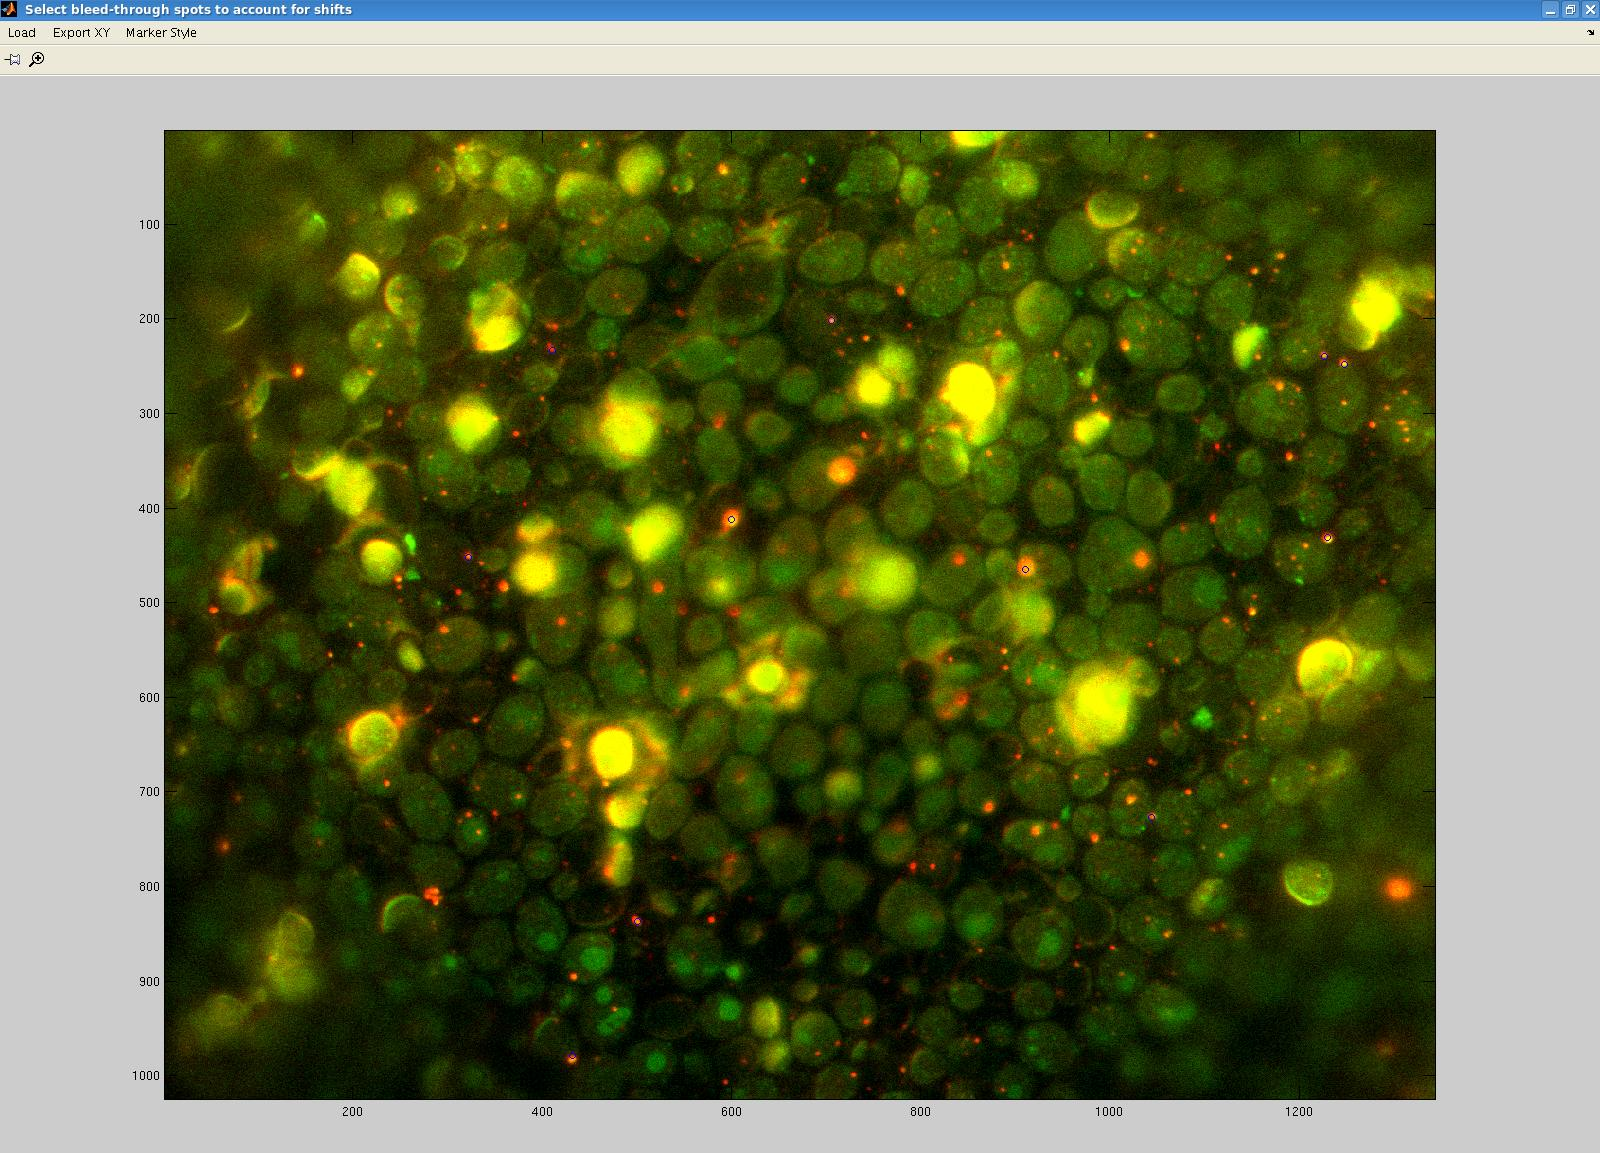
\includegraphics[width=.78\textwidth]{images/digitize.jpg}
 % digitize.jpg: 1600x1153 pixel, 762dpi, 5.33x3.84 cm, bb=0 0 151 109
 \caption{The tool for selecting the fiducials bleeding through to the fluorescence channel of interest. Clicked positions are indicated using blue circles.}
 \label{fig:digitize}
\end{figure}

\subsubsection{Calculation of the optimal transform and predicting fiducial and fluorescent spot EM-coordinates.}
Based on the set of clicked fiducials, the most accurate linear transformation (consisting of scaling, a translation and a rotation) of coordinates is calculated using the script \texttt{martin\_tfm\_beads}.
\lstinputlisting[linerange={407-408}]{../martin_correlate.m}

It scores the transformation based on all beads with the optimal transformation obtained by using a subset of beads omitting each selected fiducial pair once by comparing the sum of squares of the deviation from the predicted position of all beads with the clicked position in the EM-image.
$$
\epsilon = \frac{1}{N}\sum_{i=1}^N (T({x_{FM_i}})-x_{EMclicked_i})^2
$$
\lstinputlisting[linerange={410-411}]{../martin_correlate.m}

The resulting best coordinate transformation is applied to all cordinates and presented in a graphical output window. (Fig.\,\ref{fig:tfm_select}) The beads chosen for the transformation are displayed in the bottom left. Blue positions show the clicked coordinates in the EM-image, green dots represent the transformed position of corresponding fiducial signal from the fluorescence image. To have an idea where the spot of interest is predictted, it is shown by a magenta circle. By clicking the lower button, obiously mispicked beads can be corrected, jumping to the selection step of the algorithm.(\ref{sec:fiducials}) When clicking ``GO'', all output files will be created using the presented coordinate transformation.\\

An overlay image showing the predicted spot within the EM image as a white circle (Fig.\,\ref{fig:tfm_appl}) indicates a successful run of the collelating sript.

\begin{figure}
 \centering
 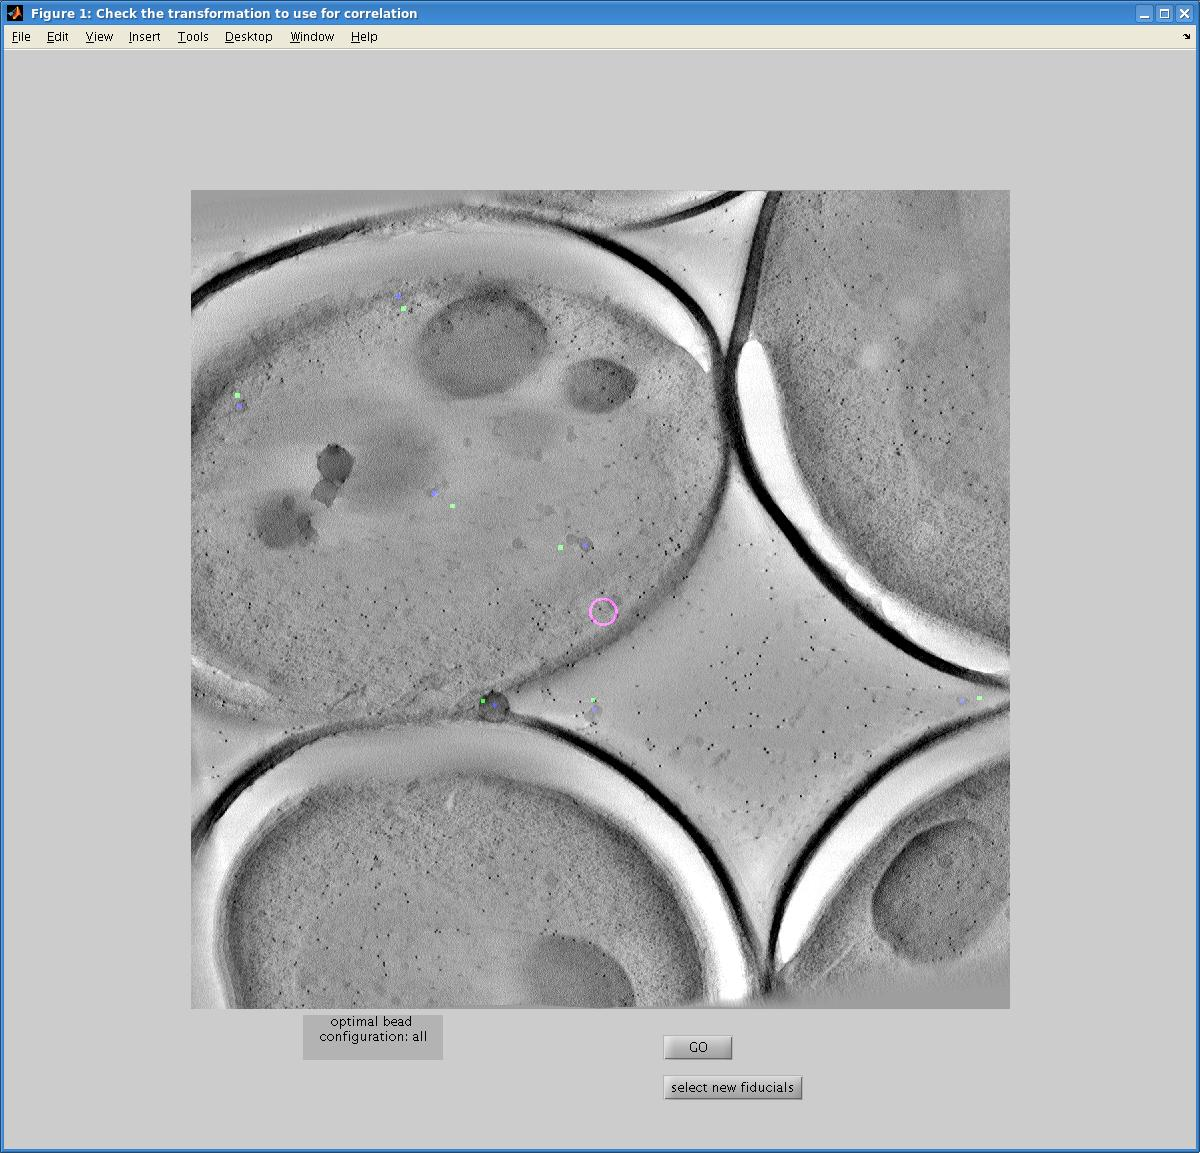
\includegraphics[width=.7\textwidth]{images/tfm_select.jpg}
 % tfm_select.jpg: 1200x1153 pixel, 762dpi, 4.00x3.84 cm, bb=0 0 113 109
 \caption{Preview of the coordinate transform. Fiducial selection can be modified by clicking the lower button.}
 \label{fig:tfm_select}
\vspace*{5mm}
 \centering
 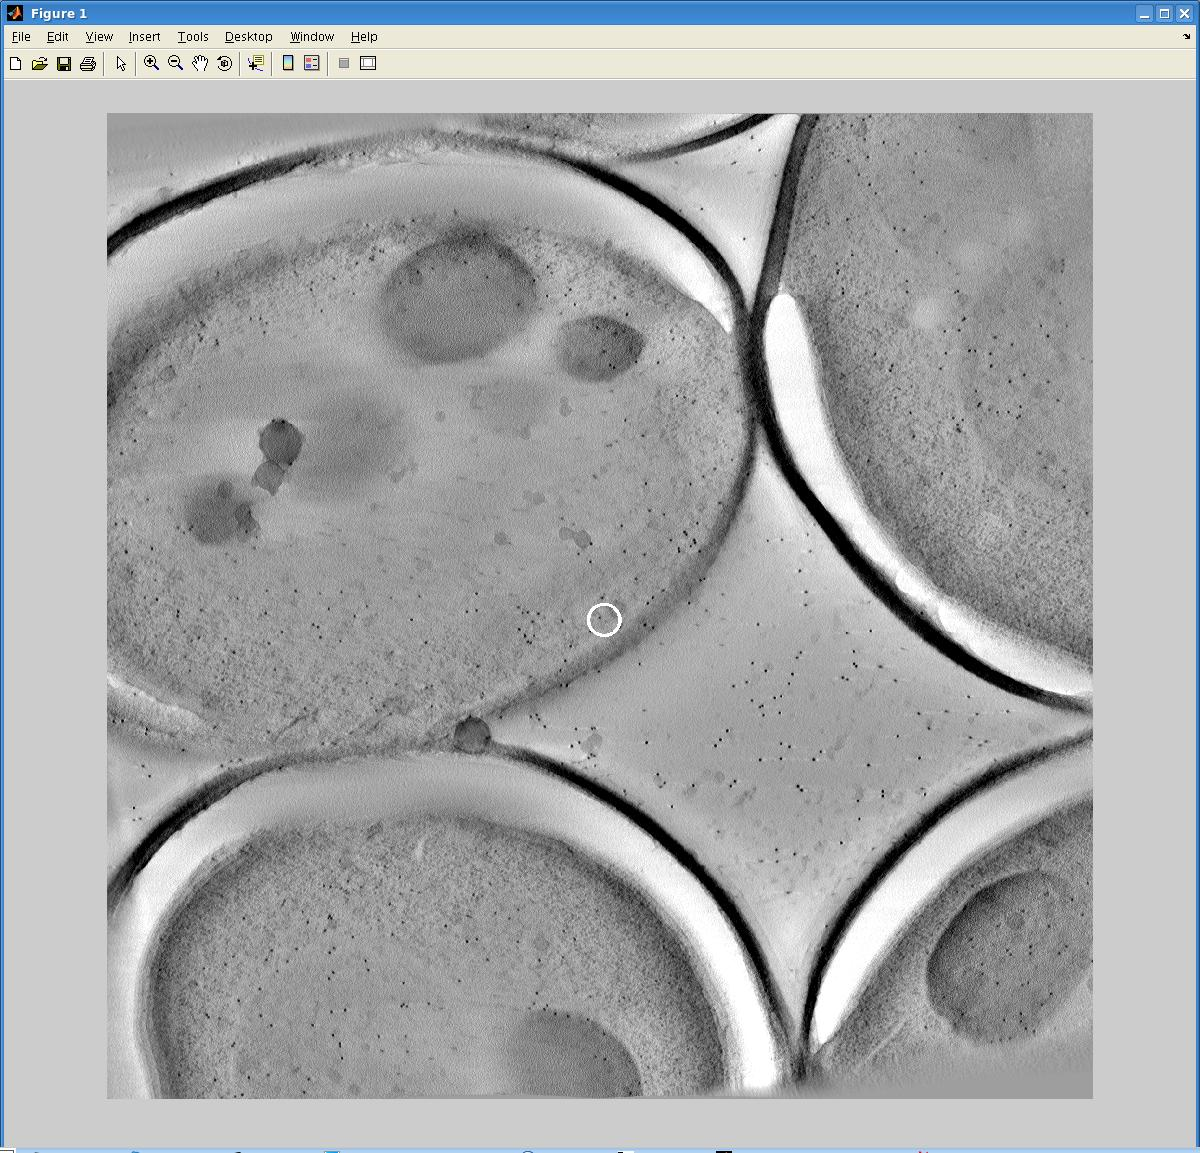
\includegraphics[width=.7\textwidth]{images/tfm_appl.jpg}
 % tfm_appl.jpg: 1200x1153 pixel, 762dpi, 4.00x3.84 cm, bb=0 0 113 109
 \caption{Performed correlation. Output position indicated by the white circle overlay.}
 \label{fig:tfm_appl}
\end{figure}
 \newpage
\section{Correlation form low magnification tomogram to high magnification EM image}

Correlation from a low resolution EM tomogram slice to a high magnification image of the same sample containing indentifiable fiducial markers such as the gold beads usesd for tomogram reconstruction is performed using the script \texttt{john\_manualregister\_LMtoHMtomo3.m}.
\subsection{Executing the script}
To execute the script and start the correlation simply run \begin{verbatim}
 martin_LMtoHM(hmf,smf,outfileroot)
\end{verbatim}
 in the MATLAB command line.

\lstinputlisting[linerange={1-8}]{../martin_LMtoHM.m}
It requires the following input parameters:
\begin{enumerate}
 \item\texttt{hmf} -- path to high mag. electron tomogram slice containing fiducial information (usually 2048$\times$2048 pixel, 8 or 16bit tiff-file)
 \item\texttt{smf} -- path to high mag. electron tomogram slice containing a probable feature of interest that is to be checked for correlation with the fluorescence signal (usually 2048$\times$2048 pixel, 8 or 16bit tiff-file)
 \item\texttt{outfileroot} -- directory and name base for generating output files.
\end{enumerate}
\subsection{Output and generated files}
The following files are generated by the correlation script during runtime. Abbreviations of file name prefixes as in \ref{sec:lm_output}. In case you require also the transformed FM images for overlays you can activate generation of those in the config script.
\begin{itemize}
\item \texttt{BASE\_XFP\_\#\_XFP.lmhmcoos.mat} -- Coordinates of fiducial marker pairs in both EM images
\lstinputlisting[linerange={41-41}]{../martin_chromaticshift_drift2.m}

\item \texttt{BASE\_XFP\_\#\_hm.tif} -- high mag. electron tomogram slice containing fiducial information 
\item \texttt{BASE\_XFP\_\#\_sm.tif} -- high mag. electron tomogram slice containing the probable feature of interest 
\item \texttt{BASE\_XFP\_\#\_XFP\_hm\_prd\_overlay.tif} -- Overlay of the prediction circle and high mag EM image containing the probable feature.


\item \texttt{BASE\_XFP\_\#\_\_XFP\_hm\_transform.log} -- Plain text log file containing the source files used for correlation, the transformed spot coordinates and information about the used transformation
\end{itemize}
\newpage
\subsection{User interaction and key procedures}
\subsubsection{Fiducial selection}
\label{sec:HM_fiducials}
A file selection dialog will ask to open the data file created by the initial correlation of the fluorescence signal.(\texttt{BASE\_XFP\_\#.appltfm.mat}) Here you have to provide a file, otherwise the script obviously cannot transform the coordinates.% After that you are asked to confirm the fluorescence channel of interest.
A file selection dialog will ask to open already existing fiducial coordinate files for the current lowMag to highMag correlation. If the selected images have never been used for correlating before, just close that window.\\

Fiducial pairs are selected in both LM and HM image using the \texttt{cpselect} tool. When an already existing coordinate file is opened, these are displayed. (Fig.\,\ref{fig:cpsel_HM}) To continue, close the window.

\begin{figure}
 \centering
 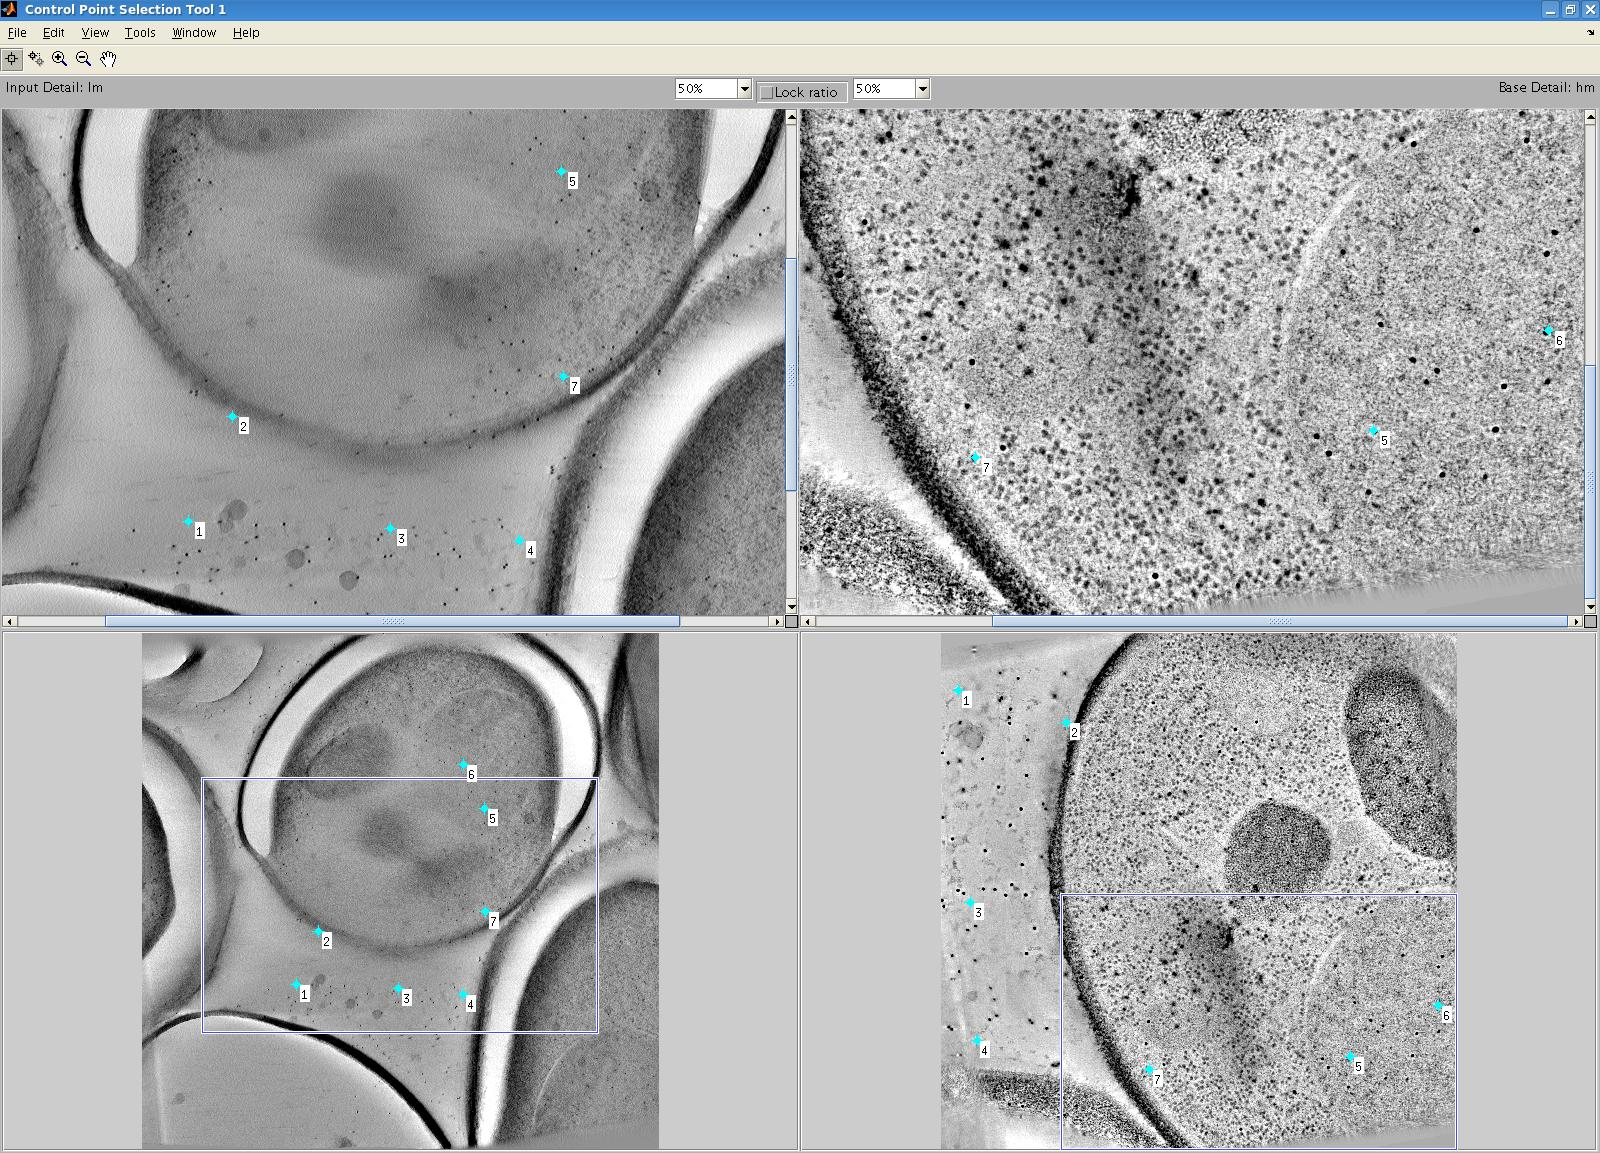
\includegraphics[width=.78\textwidth]{images/cpsel_HM.jpg}
 % cpsel_HM.jpg: 1600x1153 pixel, 72dpi, 56.44x40.68 cm, bb=0 0 1600 1153
 \caption{\texttt{cpselect} -- graphical interface for picking and checking fiducial positions}
 \label{fig:cpsel_HM}
\end{figure}

% \subsubsection{Fiducial sub-pixel fitting and display}
% Fiducial positions both image are fitted with sub-pixel accuracy using a center of mass detection.
% The fitted positions are presented again using a \texttt{cpselect} dialog. To continue, close the window.

\subsubsection{Correlation}
Coordinates are transformed using all marked fiducials and the output files are written. An overlay image showing the predicted spot within the highMag image containing the feature of interest (Fig.\,\ref{fig:tfm_HM}) indicates a successful run of the collelating sript.

\begin{figure}
 \centering
 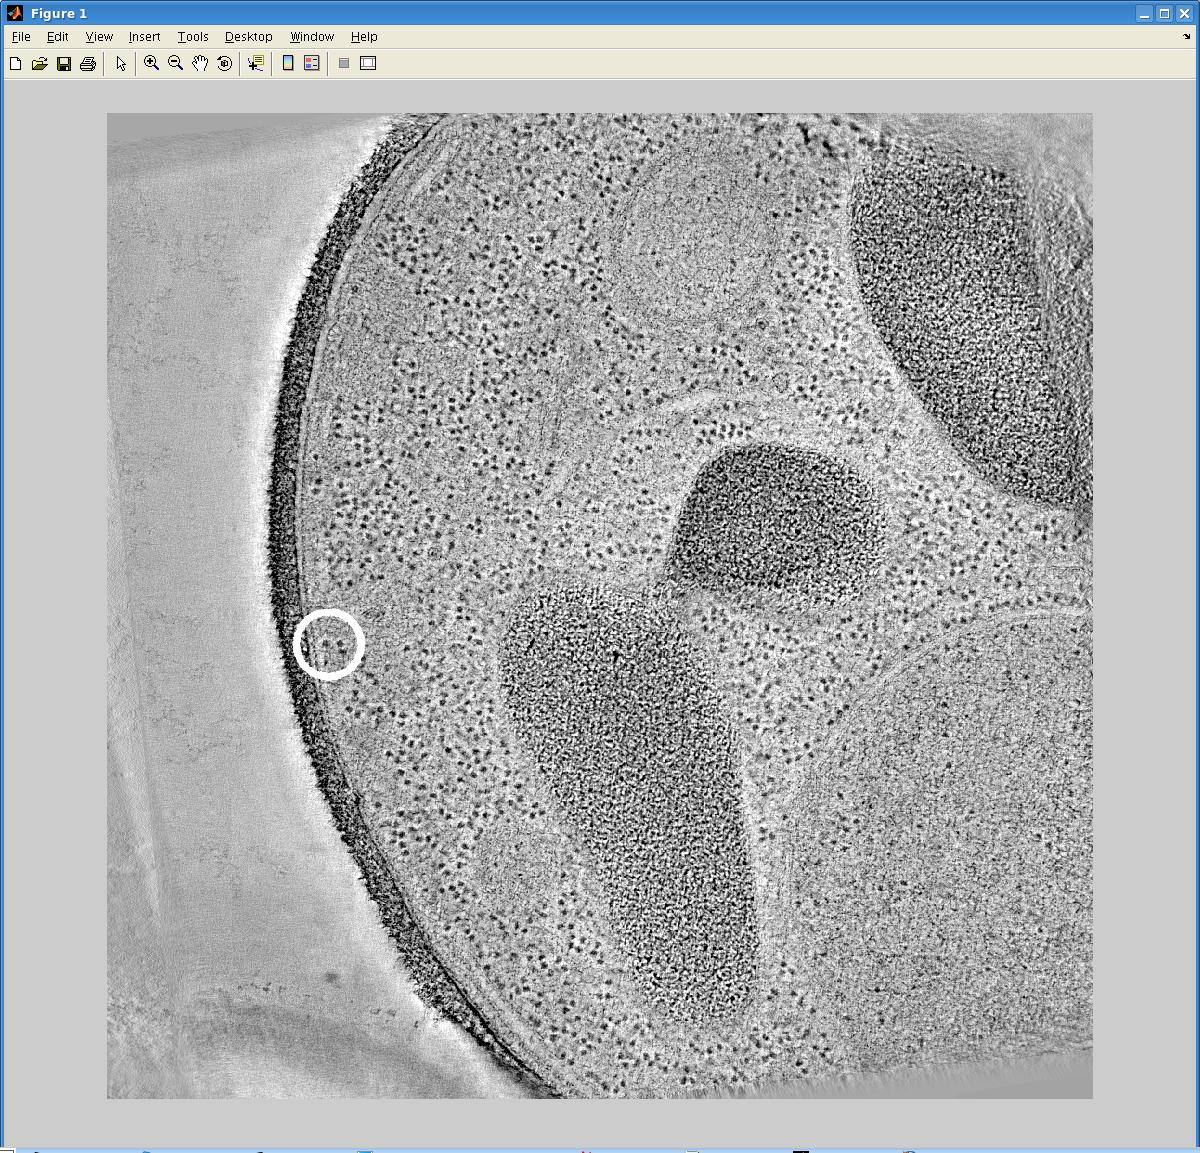
\includegraphics[width=.7\textwidth]{images/tfm_HM.jpg}
 % tfm_HM.jpg: 1200x1153 pixel, 762dpi, 4.00x3.84 cm, bb=0 0 113 109
 \caption{Performed correlation. Output position indicated by the white circle overlay.}
 \label{fig:tfm_HM}
\end{figure}

\end{document}